%% diplomovka-prezentacia.tex
%% Copyright 2016, 2017 Juraj Szasz <juraj.szasz3@gmail.com>
%
% This work may be distributed and/or modified under the conditions of the LaTeX
% Project Public License, either version 1.3 of this license or (at your option)
% any later version.  The latest version of this license is in
%   http://www.latex-project.org/lppl.txt
% and version 1.3 or later is part of all distributions of LaTeX version
% 2005/12/01 or later.
%
% This work has the LPPL maintenance status `author-maintained'.
%
% This work consists of the following files: diplomovka-prezentacia.tex,
% literatura.bib, cmidrule-patch.sty opakuj.sty, ucmplainnat.bst.
%
% The file `ucmplainnat.bst' was derived from the `csplainnat.bst' BibTeX style
% for Czech references style (According to CSN ISO 690) available at:
%   https://github.com/mudrd8mz/csplainnat
%
% All the other files above were derived from the Masaryk University, Faculty of
% Science template available for download at:
%   http://www.sci.muni.cz/NW/STUD/SablonyPraci/Sablona_Pruvodce_(v1.9).zip
%
%%%%%%%%%%%%%%%%%%%%%%%%%%%%%%%%%%%%%%%%%%%%%%%%%%%%%%%%%%%%%%%%%%%%%%%%%%%%%%%%
%%
%%  Sablona pre prezentaciu na obhajobu diplomovych prac
%%  Autor: Juraj Szasz (juraj.szasz3@gmail.com)
%%
%%  Zalozene na sablone PriF MU v Brne
%%    Autor: Petr Zemanek (zemanekp@math.muni.cz)
%%
%%  Typeset in LaTeX-2e
%%
%%%%%%%%%%%%%%%%%%%%%%%%%%%%%%%%%%%%%%%%%%%%%%%%%%%%%%%%%%%%%%%%%%%%%%%%%%%%%%%%

\documentclass{beamer}
\usetheme{Warsaw}      % pouzitie temy Warsaw

\usepackage[utf8]{inputenc}
\usepackage[IL2]{fontenc}
\usepackage[english,slovak]{babel} % posledny jazyk v zozname je implicitny

\usepackage{booktabs}  % balík pre vysadzanie profesionalnych tabuliek

\usepackage{amsmath,amssymb,amsthm} % baliky pre matematicke vzorce
\usepackage{natbib}    % balik pre harvardsky styl citacii

\usepackage{tikz}      % balik pre zmenu opacity objektov
\usepackage{color, colortbl} % balik pre definiciu vlastnych farieb
\definecolor{LRed}{rgb}{1,.8,.8}

% Nastavenie obrazku na pozadi
\usebackgroundtemplate{%
  \tikz\node[opacity=0.05]{\parbox{\paperwidth}{\centering
\includegraphics[height=\paperheight]{logo/UCM_(color).png}}};
}


%%%%%%%%%%%%%%%%%%%%%%%%%%%%%%%%%%%%%%%%%%%%%%%%%%%%%%%%%%%%%%%%%%%%%%%%%%%%%%%%
%%
%%  Nastavenie stylu citacii
%%
%%%%%%%%%%%%%%%%%%%%%%%%%%%%%%%%%%%%%%%%%%%%%%%%%%%%%%%%%%%%%%%%%%%%%%%%%%%%%%%%
\bibliographystyle{ucmplainnat}
\setcitestyle{authoryear}

%%%%%%%%%%%%%%%%%%%%%%%%%%%%%%%%%%%%%%%%%%%%%%%%%%%%%%%%%%%%%%%%%%%%%%%%%%%%%%%%
%%
%%  Nastavenie sablony
%%
%%%%%%%%%%%%%%%%%%%%%%%%%%%%%%%%%%%%%%%%%%%%%%%%%%%%%%%%%%%%%%%%%%%%%%%%%%%%%%%%

\graphicspath{{obr/}}                 % implicitna cesta pre umiestnenie
                                      % obrazkov v adresari 'obr'

\author{Bc. Juraj Szász}              % autor

% Afiliacia a dodatocne info na titulny slajd
\institute{\begin{tabular}{l@{\hspace{0.5em}}l}
  \textbf{Študijný program:} & Aplikovaná biológia \\
  \textbf{Študijný obor:}  & Biológia \\
  \textbf{Školiace pracovisko:} & Katedra biológie \\
  \textbf{Školiteľ:} & prof. RNDr. Ján Kraic, PhD \\
 \end{tabular}
 \\ \vspace{10pt}  \textcolor{blue}{Fakulta prírodných vied} \\
 \textcolor{blue}{\textbf{Univerzita sv.\,Cyrila a Metoda v Trnave}}}

% Nazov prezentacie
\title{Scientometrická analýza FPV~UCM v~Trnave}

% Podtitulok prezentacie
\subtitle{Diplomová práca}

% Datum
\date{25.\,januára 2017}

\setbeamercovered{transparent}

%%%%%%%%%%%%%%%%%%%%%%%%%%%%%%%%%%%%%%%%%%%%%%%%%%%%%%%%%%%%%%%%%%%%%%%%%%%%%%%%
%%
%% Definícia vlastných príkazov
%%
%%%%%%%%%%%%%%%%%%%%%%%%%%%%%%%%%%%%%%%%%%%%%%%%%%%%%%%%%%%%%%%%%%%%%%%%%%%%%%%%

\newcommand{\tm}{\texttrademark}
\newcommand{\R}{\textsuperscript{\textregistered}}

% Environment for source code
\newenvironment{source}[1][\scriptsize\bfseries]{
  \begin{list}{}{
      \setlength{\leftmargin}{1em}}%
      \setlength{\itemsep}{0pt}%
      \setlength{\parskip}{0pt}%
      \setlength{\parsep}{0pt}%
      \renewcommand{\baselinestretch}{1.0}%
  \item#1}
  {\end{list}}
%%%%%%%%%%%%%%%%%%%%%%%%%%%%%%%%%%%%%%%%%%%%%%%%%%%%%%%%%%%%%%%%%%%%%%%%%%%%%%%%
%%
%%  Dodatocne nastavenia
%%
%%%%%%%%%%%%%%%%%%%%%%%%%%%%%%%%%%%%%%%%%%%%%%%%%%%%%%%%%%%%%%%%%%%%%%%%%%%%%%%%

% Zapnutie opakovania matematickych symbolov
% %Podle Tesaříkova czech.ldf
\makeatletter
\def\Deleni{%
 \ifx\protect\@typeset@protect
   \ifhmode
     \ifinner
       \bbl@afterelse\bbl@afterelse\bbl@afterelse\cs@hyphen
     \else
       \bbl@afterfi\bbl@afterelse\bbl@afterelse\cs@firsthyphen
     \fi
   \else
     \bbl@afterfi\bbl@afterelse\cs@hyphen
   \fi
 \else
   \bbl@afterfi\cs@hyphen
 \fi }
\makeatother

%Opakování symbolů binárních operací a relací při zalomení řádku
%Autor: Josef Tkadlec tkadlec@fel.cvut.cz

\relpenalty     =10000      % aby se nelámalo v jiných než ošetřených
\binoppenalty   =10000
\exhyphenpenalty=1000       % aby spíše nouzově (implicitně je 50)
                           % "lokálně" lze zakázat {...}

\def\neq {\mathrel{\not=}}  % aby nedocházelo k lámání \not=/=
\let\ne=\neq

\def\OpakujPrikaz #1#2{\let #2=#1
 \def #1{#2\nobreak\discretionary{}{\hbox{$#2$}}{}}}
\def\OpakujZnak #1#2{\mathchardef #2=\mathcode`#1
 \activedef #1{#2\nobreak\discretionary{}{\hbox{$#2$}}{}}
 \uccode`\~=0 \mathcode`#1="8000 }
%Doplnil Kuben pro nový czech.ldf \expandafter možná nemusí být
\def\OpakujZnakMinus #1#2{\mathchardef #2=\mathcode`#1
 \activedef #1{\ifmmode#2\nobreak\discretionary{}{\hbox{$#2$}}{}\else\expandafter\Deleni\fi }
 \uccode`\~=0 \mathcode`#1="8000 }
\def\activedef #1{\uccode`\~=`#1 \uppercase{\def~}}

\OpakujPrikaz {\neq }{\neqORI}  \let \ne=\neq
\OpakujPrikaz {\leq }{\leqORI}  \let \le=\leq
\OpakujPrikaz {\geq }{\geqORI}  \let \ge=\geq
\OpakujPrikaz {\cup }{\cupORI}
\OpakujPrikaz {\cap }{\capORI}
\OpakujPrikaz {\times }{\timesORI}
\OpakujPrikaz {\subset }{\subsetORI}
\OpakujPrikaz {\subseteq }{\subseteqORI}
\OpakujPrikaz {\supset }{\supsetORI}
\OpakujPrikaz {\supseteq }{\supseteqORI}

\OpakujPrikaz {\cdot }{\cdotORI}
\OpakujPrikaz {\setminus }{\setminusORI}

\OpakujZnak <{\lessORI}
\OpakujZnak >{\greaterORI}
\OpakujZnak +{\plusORI}
\AtBeginDocument {\OpakujZnak ={\eqORI} \OpakujZnakMinus -{\minusORI}}

% Prikaz \cmidrule nefunguje, ak dokument pouziva slovencinu/cestinu cez babel
% tento patch riesi tento problem
\begingroup
    \makeatletter
    \catcode`\-=\active
    \AtBeginDocument{
    \def\@@@cmidrule[#1-#2]#3#4{\global\@cmidla#1\relax
        \global\advance\@cmidla\m@ne
        \ifnum\@cmidla>0\global\let\@gtempa\@cmidrulea\else
        \global\let\@gtempa\@cmidruleb\fi
        \global\@cmidlb#2\relax
        \global\advance\@cmidlb-\@cmidla
        \global\@thisrulewidth=#3
        \@setrulekerning{#4}
        \ifnum\@lastruleclass=\z@\vskip \aboverulesep\fi
        \ifnum0=`{\fi}\@gtempa
        \noalign{\ifnum0=`}\fi\futurenonspacelet\@tempa\@xcmidrule}
    }
\endgroup


%%%%%%%%%%%%%%%%%%%%%%%%%%%%%%%%%%%%%%%%%%%%%%%%%%%%%%%%%%%%%%%%%%%%%%%%%%%%%%%%
%%
%%  Zaciatok dokumentu
%%
%%%%%%%%%%%%%%%%%%%%%%%%%%%%%%%%%%%%%%%%%%%%%%%%%%%%%%%%%%%%%%%%%%%%%%%%%%%%%%%%

\begin{document}

%%
%%  Titulny slajd
%%
\frame{\maketitle}


%%
%%  Osnova
%%
\frame{\tableofcontents}


\section[Úvod]{Úvod}

\subsection{Definícia scientometrie}

%
%  Definicia scientometrie
%
\begin{frame}{Čo je scientometria?}
  \begin{block}{Definícia scientometrie}
    Scientometria je hodnotenie vedy (publikácií, pracovníkov, inštitúcií, až
    krajín) použitím matematických a štatistickým metód \citep{Vinkler2001}.
  \end{block}
  \begin{itemize}
    \item Základ hodnotenia tvorí počet referencií na publikáciu tzv. citácie.
      Pričom táto hodnota predstavuje impakt (dopad) daného dokumentu na vedu,
      teda kvalitu \citep{Vavrikova2008}.
    \item V scientometrie sa môže hodnotiť aj ekonomický aspekt vedeckého
      výskumu (napr. financovanie inštitúcií a grantov), ale väčšiu váhu má
      hodnote nie na základe citácií, pretože financovanie samo o sebe nič
      nehovorí o dopade daného objavu \citep{Bellis2009}.
  \end{itemize}
\end{frame}


%\subsection{Citačné registre (Scopus, Web of Science, Google Scholar)}

%
% Citačné registre: Scopus
%
%\begin{frame}{Scopus}
%  Contents\dots
%\end{frame}

%
% Citačné registre: Web of Science
%
%\begin{frame}{Web of Science}
%  Contents\dots
%\end{frame}

%
% Citačné registre: Google Scholar
%
%\begin{frame}{Google Scholar}
%  Contents\dots
%\end{frame}


\subsection{Citačné indikátory}

%
% Prehlad citacnych indikatorov
%
\begin{frame}{Prehľad citačných indikátorov}
  \begin{table}
    \centering\footnotesize
    \begin{tabular}{llcr}
      \toprule
      slovenský názov & anglický názov & skratka & kap. \\
      \midrule
      \rowcolor{LRed} impakt faktor                 & \emph{Journal Impact Factor}    & IF        & 1.5.1 \\[0.5ex]
      \rowcolor{LRed} SciMago rang časopisu         & \emph{SciMago Journal Rank}     & SJR       & 1.5.2 \\[0.5ex]
      \rowcolor{LRed} CiteScore$^\dagger$            & \emph{CiteScore}                & CS        & 1.5.3 \\[0.5ex]
      \rowcolor{LRed} normalizovaný impakt časopisu & \emph{Source normalized impact} & SNIP      & 1.5.4 \\[-0.25ex]
      \rowcolor{LRed} na dokument                   & \emph{per paper}                &           &       \\[0.5ex]
      Hirschov index                                & \emph{Hirsh's index}            & $h$-index & 1.6.1 \\[1.5ex]
      Eggheov index                                 & \emph{Egghe's index}            & $g$-index & 1.6.2 \\[0.5ex]
      \bottomrule
      \multicolumn{4}{l}{\tiny {\color{red} červenou farbou} sú označené citačné indikátory na hodnotenie časopisov} \\
      \multicolumn{4}{l}{\tiny $^\dagger$ indikátory, ktorých názov sa neprekladá so slovenčiny}
    \end{tabular}
  \end{table}
\end{frame}


\section{Ciele práce}

%%
%% Ciele prace
%%
\begin{frame}{Ciele práce}
  \begin{enumerate}
  \item<1-> Získať bibliografické záznamy všetkých publikácií každého vedeckého
    pracovníka, ktorý je uvedený na stránkach fakulty FPV UCM v Trnave a na
    stránkach príslušných katedier.
  \item<2-> Získať bibliografické záznamy pre práce, v ktorých má aspoň jeden
    spoluautor príslušnosť FPV UCM v Trnave.
  \item<3-> Urobiť citačnú analýzu vedeckých publikácií pracovníkov FPV UCM v
    Trnave.
  \item<4-> Rozdeliť citačné analýzy jednotlivých pracovníkov podľa príslušnosti
    ku katedrám a vytvoriť sumárne citačné analýzy pre každú katedru.
  \item<5-> Graficky zhodnotiť a porovnať výsledok citačných analýz pre každu
    katedru a graficky zhodnotiť vývoj publikačnej činnosti FPV UCM v Trnave.
  \end{enumerate}
\end{frame}


\section{Materiály a metódy}

%\subsection{Získavanie dát}

%
% Ziskavanie dat: Scopus
%
%\begin{frame}{Scopus}
%  Contents\dots
%\end{frame}

%
% Ziskavanie dat: Web of Sciencee
%
%\begin{frame}{Web of Science}
%  Contents\dots
%\end{frame}


\subsection{Analýza pracovníkov}

%
% Analyza pracovnikov: Zoznam pracovnikov
%
\begin{frame}{Rozdelenie pracovníkov do kadetier}

  \begin{table}
    \centering\small
    \begin{tabular}{llc}
      \toprule%\noalign{\vspace{.3ex}}
      Názov katedry                   & Skr.    & $n$\\%[0.3ex]
      \midrule%\noalign{\vspace{.5ex}}
      Katedra biológie                & KB      & 13 \\%[0.5ex]
      Katedra biotechnológií          & KBt     & 10 \\%[0.5ex]
      Katedra chémie                  & KCh     & 18 \\%[0.5ex]
      Katedra ekochémie               & KER     & 6 \\[-0.25ex]
      a rádiobiológie                 &         &                                             \\ [0.5ex]
      Kat. aplikovanej informatiky    & KAIM    & 14 \\%[-0.25ex]
      a matematiky                    &         &                                              \\[0.5ex]
      Katedra biofyziky               & KBf     & 6 \\%[0.5ex]
      Katedra odbornej jazykovej      & KOIP    & 2 \\[-0.25ex]
      prípravy                        &         &                                              \\[0.5ex]
      \bottomrule
    \end{tabular}
  \end{table}


\end{frame}

%
% Analyza pracovnikov: Chybajuce data
%
%\begin{frame}{Chýbajúce dáta}
%Contents\dots
%\end{frame}


\subsection{Program Publish or Perish}

%
% Screenshot programu Publish or Perish
%
\begin{frame}{Program Publish or Perish}
  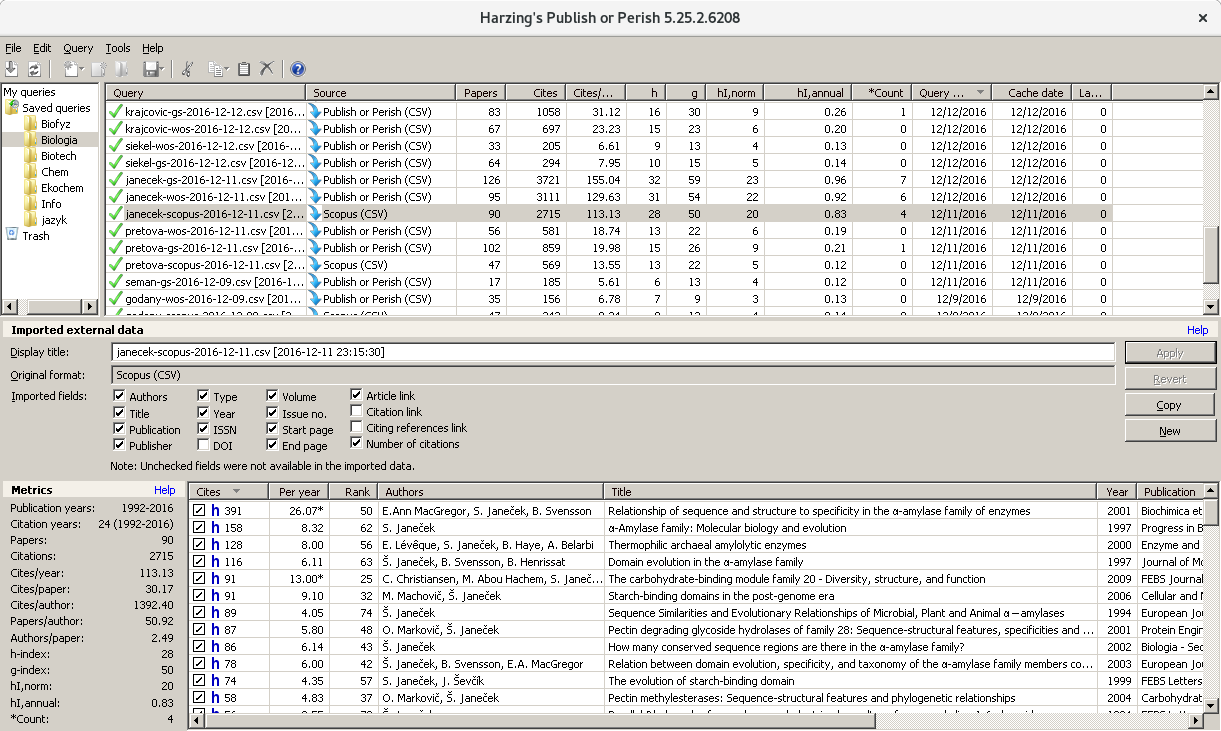
\includegraphics[scale=0.255]{publish-or-perish_wine.png} \\[-1ex]
  \parbox{\textwidth}{\centering\tiny \citet{Harzing2011}}
\end{frame}


%\subsection{Vlastné programy na spracovanie dát}

%
% Popis vlastnych programov na spracovanie dat
%
%\begin{frame}{Vlastné programy na spracovanie dát}
%  \begin{block}{scientometry-data-proc}
%    Contents\dots
%  \end{block}

%  \begin{block}{scientometry-plot-gen}
%    Contents\dots
%  \end{block}
%\end{frame}


\section{Výsledky a diskusia}

\subsection{Celkový počet publikácii a citácii jednotlivých katedier}

%
% Graf celkoveho poctu publikacii jednotlivých katedier
%
\begin{frame}{Celkový počet publikácii jednotlivých katedier FPV}
  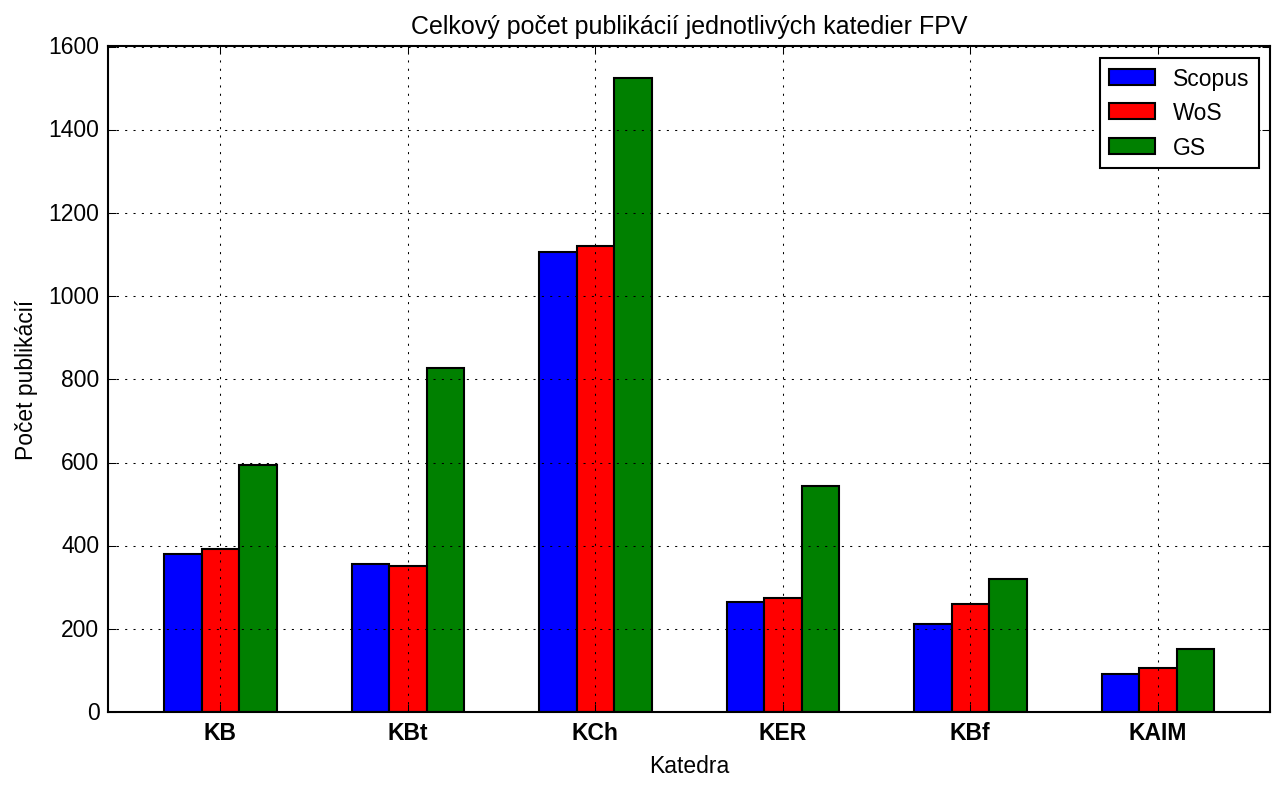
\includegraphics[scale=0.5]{plot-results-data-papers.png}
\end{frame}

%
% Graf celkoveho poctu citacii jednotlivych katedier
%
\begin{frame}{Celkový počet citácií jednotlivých katedier FPV}
  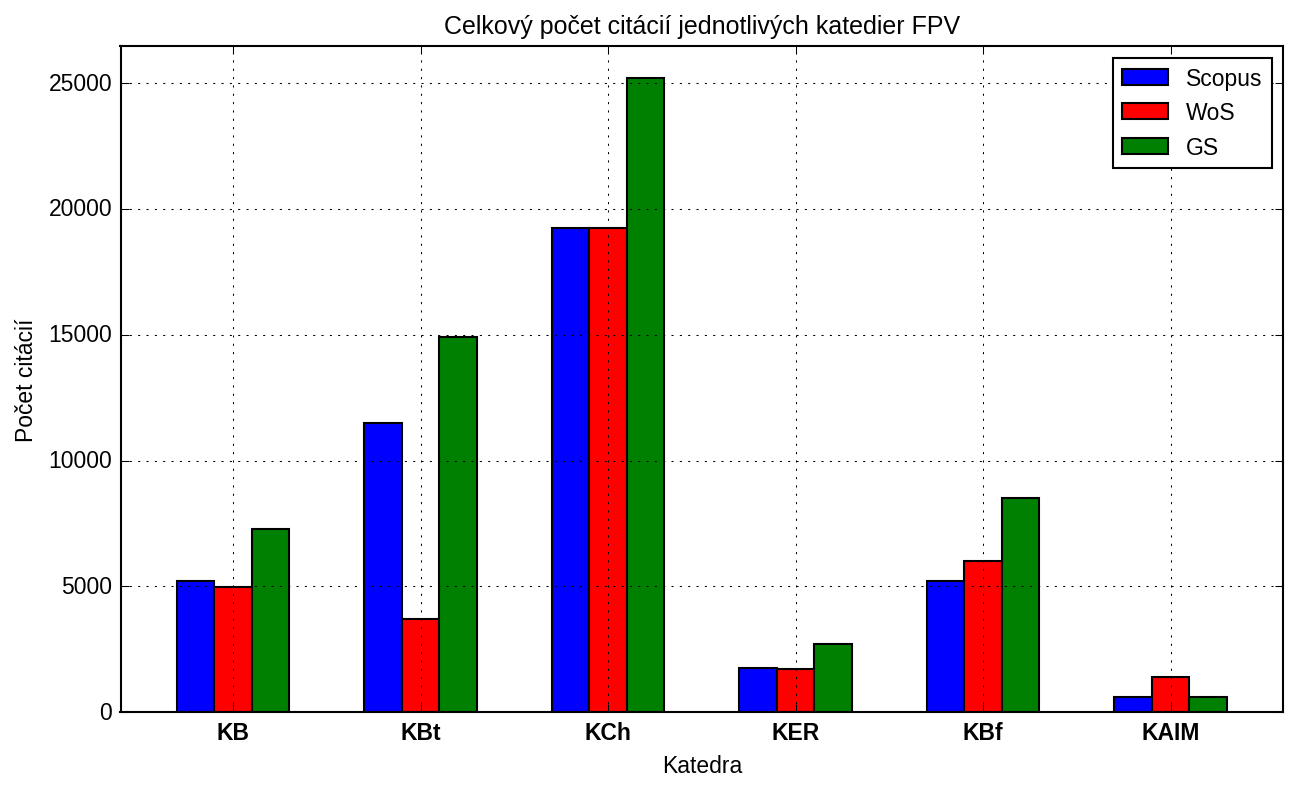
\includegraphics[scale=0.5]{plot-results-data-citations.png}
\end{frame}


\subsection{Medián vybraných citačných indikátorov pre jednotlivé katedry}
%
% Graf h-indexu pre jednotlive katedry
%
\begin{frame}{Medián $h$-indexu pre jednotlivé katedry FPV}
  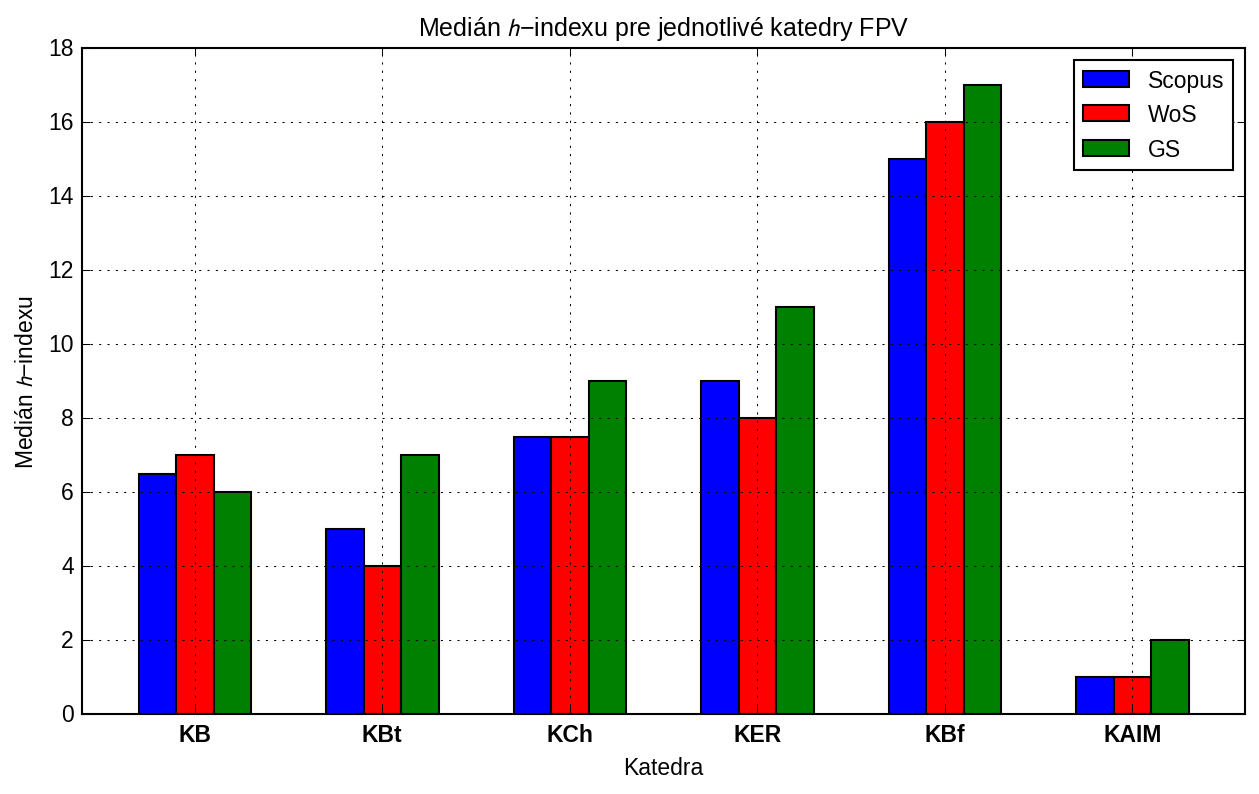
\includegraphics[scale=0.5]{plot-results-data-h_index.png}
\end{frame}

%
% Graf g-indexu pre jednotlive katedry
%
\begin{frame}{Medián $g$-indexu pre jednotlivé katedry FPV}
  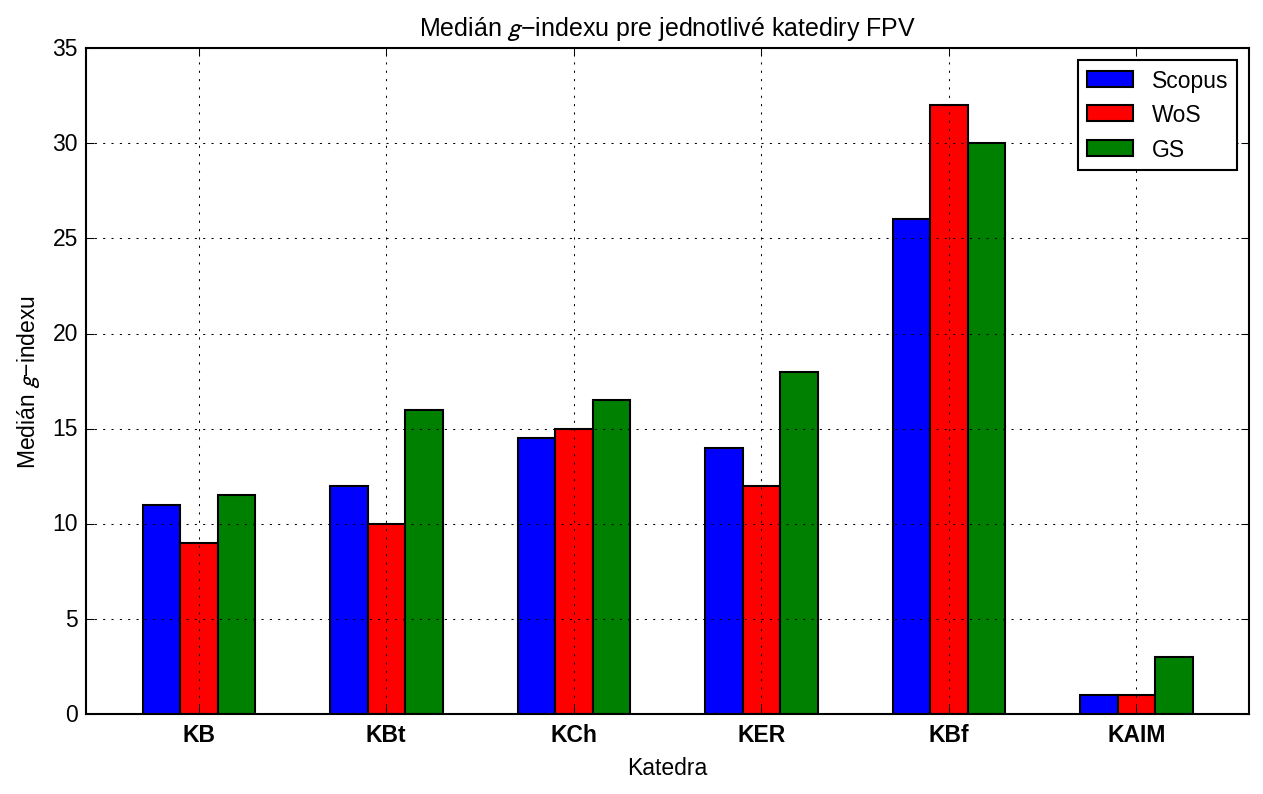
\includegraphics[scale=0.499]{plot-results-data-g_index.png}
\end{frame}

\subsection{Porovnanie KCh FPV s gréckymi univerzitami}

%
% KCh FPV vs. katedra chemickeho inzinierstva troch greckych univerzit
%
\begin{frame}{Porovnanie KCh FPV s katedrami chemického inžinierstva vybraných troch gréckych univerzít}
  \begin{table}
    \footnotesize
    \begin{tabular}{lccclccc}
      \toprule
      & \multicolumn{3}{c}{Katedra chémie FPV} & & \multicolumn{3}{c}{\citet{Kazakis2015}} \\
      \cmidrule{2-4}\cmidrule{6-8}
      Indikátor & Scopus & WoS & GS & & Atény$^{\mathrm{a}}$ & Solún$^{\mathrm{a}}$ & Patra$^{\mathrm{a}}$ \\
      \midrule
      $n$            & 18    & 18    & 18    & & 72    & 34    & 30    \\
      $P$            & 1106  & 1120  & 1525  & & 4463  & 2253  & 2573  \\
      P/A$^\dagger$  & 15,42 & 16,14 & 25,74 & & 62    & 66,3  & 85,8  \\
      $c$            & 19248 & 19223 & 25208 & & 74368 & 39695 & 63718 \\
      C/P$^\ddagger$ & 12,45 & 12,62 & 11,35 & & 16,7  & 17,6  & 24,8  \\
      $\bar{h}$      & 11,78 & 11,94 & 13,61 & & 16,3  & 16,8  & 21,3  \\
      $\sigma (h)$   & 11,70 & 11,70 & 12,99 & & 8     & 8,5   & 1,5   \\
      $\tilde{h}$    & 7,50  & 7,50  & 9,00  & & 15,5  & 17    & 18    \\
      $\bar{g}$      & 19,83 & 20,22 & 23,56 & & 26,8  & 28,3  & 35,5  \\
      $\sigma (g)$   & 22,23 & 21,68 & 24,89 & & 12,6  & 13,9  & 23    \\
      $\tilde{g}$    & 14,50 & 15,00 & 16,50 & & 26,5  & 27    & 30,5  \\
      \bottomrule
      \multicolumn{8}{l}{\tiny $^\dagger$ počet autorov na publikáciu; $^\ddagger$ počet citácii na publikáciu; $^{\mathrm{a}}$ zdroj: Scopus}
    \end{tabular}
  \end{table}
\end{frame}

%
% KCh FPV vs. katedra chemie vybranych piatich greckych univerzit
%
\begin{frame}{Porovnanie KCh FPV s katedrami chémie vybraných piatich gréckych univerzít}
  \begin{table}
    \footnotesize
    \begin{tabular}{lccc}
    \toprule
    & \multicolumn{3}{c}{Katedra chémie FPV} \\
    \cmidrule{2-4}
    Indikátor & Scopus & WoS & GS \\
    \midrule
    $P$        & 1106   & 1120  & 1525  \\
    $\bar{h}$  & 11,78  & 11,94 & 13,61 \\
    \bottomrule
    \end{tabular}
  \end{table}
  \begin{table}
    \footnotesize
    \begin{tabular}{lccccc}
    \toprule
    & \multicolumn{5}{c}{\citet{Lazaridis2010}} \\
    \cmidrule{2-6}
    Indikátor & Kréta & Patra & Solún & Ioaninna & Atény \\
    \midrule
    $P$        & 56    & 61    & 41    & 48       & 219   \\
    $\bar{h}$  & 16,6  & 12,6  & 10,4  & 10,3     & 9,0   \\
    \bottomrule
    \end{tabular}
  \end{table}
\parbox{\textwidth}{\centering\tiny Zdroj: Web of Science}
\end{frame}

\subsection{Časopisy s najväčším počtom publikácii z FPV}

%
% Tabulka casopisov s najvacsim poctom publikacii
%
\begin{frame}{Svetové časopisy s najväčším počtom publikácii z FPV}
\begin{table}
  {\footnotesize
  \begin{tabular}{lccccc}
    \toprule
     Názov časopisu & $n^\dagger$ & IF & SJR  & CS$^\ddagger$ & SNIP \\
    \midrule
    Chemical Papers                 & 25 & 1,326 & 0,382 & 1,36 & 0,56  \\
    Polyhedron                      & 22 & 2,108 & 0,592 & 2,02 & 0,777 \\
    Biologia                        & 15 & 1,10  & 0,322 & 0,88 & 0,88  \\
    Cereal Research Communications  & 14 & 0,528 & 0,305 & 0,62 & 0,515 \\
    Dalton Transactions             & 14 & 4,177 & 1,404 & 4,1  & 1     \\[1ex]
    Chemicke Listy                  & 13 & 0,279 & 0,183 & 0,22 & 0,24  \\
    Inorganic Chemistry             & 12 & 4,82  & 1,873 & 1,36 & 0,741 \\
    Inorganica Chimica Acta         & 11 & 1,918 & 0,584 & 1,88 & 0,664 \\
    Nova Biotechnologica et Chimica & 11 & 0,188 & 0,129 & 0,31 & 0,044 \\
    \bottomrule \\[-2ex]
    \multicolumn{6}{l}{\tiny $^\dagger$ Počet publikácií pracovníkov FPV; $^\ddagger$ CiteScore} \\
  \end{tabular}}
\end{table}
\parbox{\textwidth}{\centering\tiny Zdroj: Scopus a Web of Science (2000-2016)}
\end{frame}


\section{Záver}

%%
%% Zaver
%%
\begin{frame}{Záver}
  \begin{itemize}
  \item<1-> Z technických dôvodov sme do analýz nezahrnuli odstránenie
    autocitácií.
  \item<2-> Práca nezahŕňa výpočet spoluatorských sietí, pretože by tak
    presiahla predpísaný rozsah.
  \item<3-> I napriek sa nám v rámci možností podarilo splniť stanovené ciele.
  \item<4-> Táto práca tak predstavuje prvú komplexnejšiu scientometrickú
    analýzu FPV UCM v Trnave a môže sa stať užitočným podkladom pre ďaľšie práce
    tohto typu.
  \end{itemize}
\end{frame}

% ------------------------------------------------------------------------------

%%
%% Dodatky
%%
\appendix

%
% Podakovanie
%
\begin{frame}
  \begin{center}
    \Huge Ďakujem za pozornosť!
    \vfill
    \Large Juraj Szász
  \end{center}
\end{frame}

%
% Zoznam literatury
%
\begin{frame}[t, allowframebreaks]
  \frametitle{Zoznam literatúry}
  \bibliography{literatura}{}
\end{frame}

%
% Reakcie na otazky oponenta
%
\section{Reakcia na otázky oponenta}

\subsection{Iné zdroje impakt faktoru}

\begin{frame}{Iné zdroje impakt faktoru}
  \begin{table}
    \centering\footnotesize
    \begin{tabular}{lccl}
      \toprule
      Časopis & ISI JIF & IF & Zdroj \\
      \midrule
      Polish Journal of Enviromental Studies   & 0,79  & 0,71           & Research Gate$^{\mathrm{a}}$ \\[0.5ex]
      Pharmazie                                & 1,264 & 1,32           & Research Gate$^{\mathrm{b}}$ \\[0.5ex]
      Applied Mechanics and Materials          & --    & 0,16           & Research Gate$^{\mathrm{c}}$ \\[0.5ex]
      Advanced Materials Research              & --    & 0,23           & Research Gate$^{\mathrm{d}}$ \\[0.5ex]
      Nova Biotechnologica et Chimica          & --    & 0,188$^\dagger$ & De Gruyter$^{\mathrm{e}}$    \\[0.5ex]
      Communications in Comp. and Inf. Science & --    & 0,35           & Research Gate$^{\mathrm{f}}$ \\[0.5ex]
      \bottomrule
      \multicolumn{4}{l}{\tiny $^\dagger$ Hodnota nie je impakt faktor, ale impakt na publikáciu (IPP)} \\
      \multicolumn{4}{l}{\tiny $^{\mathrm{a}}$ \url{https://www.researchgate.net/journal/1230-1485\_Polish\_Journal\_of\_Environmental\_Studies}} \\
      \multicolumn{4}{l}{\tiny $^{\mathrm{b}}$ \url{https://www.researchgate.net/journal/0031-7144\_Pharmazie}} \\
      \multicolumn{4}{l}{\tiny $^{\mathrm{c}}$ \url{https://www.researchgate.net/journal/1660-9336\_Applied\_Mechanics\_and\_Materials}} \\
      \multicolumn{4}{l}{\tiny $^{\mathrm{d}}$ \url{https://www.researchgate.net/journal/1662-8958\_Advanced\_Materials\_Research}} \\
      \multicolumn{4}{l}{\tiny $^{\mathrm{e}}$ \url{https://www.degruyter.com/view/j/nbec}} \\
      \multicolumn{4}{l}{\tiny $^{\mathrm{f}}$ \url{https://www.researchgate.net/journal/1865-0929\_Communications\_in\_Computer\_and\_Information\_Science}} \\
    \end{tabular}
  \end{table}
\end{frame}

\end{document}
